\usepackage[utf8]{inputenc}       
\usepackage[T1]{fontenc}          
\usepackage[italian]{babel}       
\usepackage{graphicx}             
\usepackage{float}
\usepackage{amsmath}
\usepackage{amsfonts} 
\usepackage{amssymb}  
\usepackage{steinmetz}
\usepackage{pgfplots}
\usepackage{tikz}
\usepackage{enumitem} 
\usepackage{subcaption}
\usepackage{caption}
\usepackage[normalem]{ulem}
\usepackage[americaninductors, siunitx]{circuitikz}

\usetikzlibrary{arrows.meta, patterns, shapes.geometric, calc, positioning, shapes, arrows}
\pgfplotsset{compat=1.18}

% --- GEOMETRY (Margini e distanze) ---
\usepackage[
    a4paper,
    top=3.5cm,      
    bottom=3cm,    
    left=3cm,      
    right=3cm,     
    headheight=40pt, % Spazio per l'immagine
    headsep=25pt     % Distanza tra immagine e testo/titoli
]{geometry}

% --- FANCYHDR (Intestazioni) ---
\usepackage{fancyhdr} 
\pagestyle{fancy}
\fancyhf{} 
\fancyhead[L]{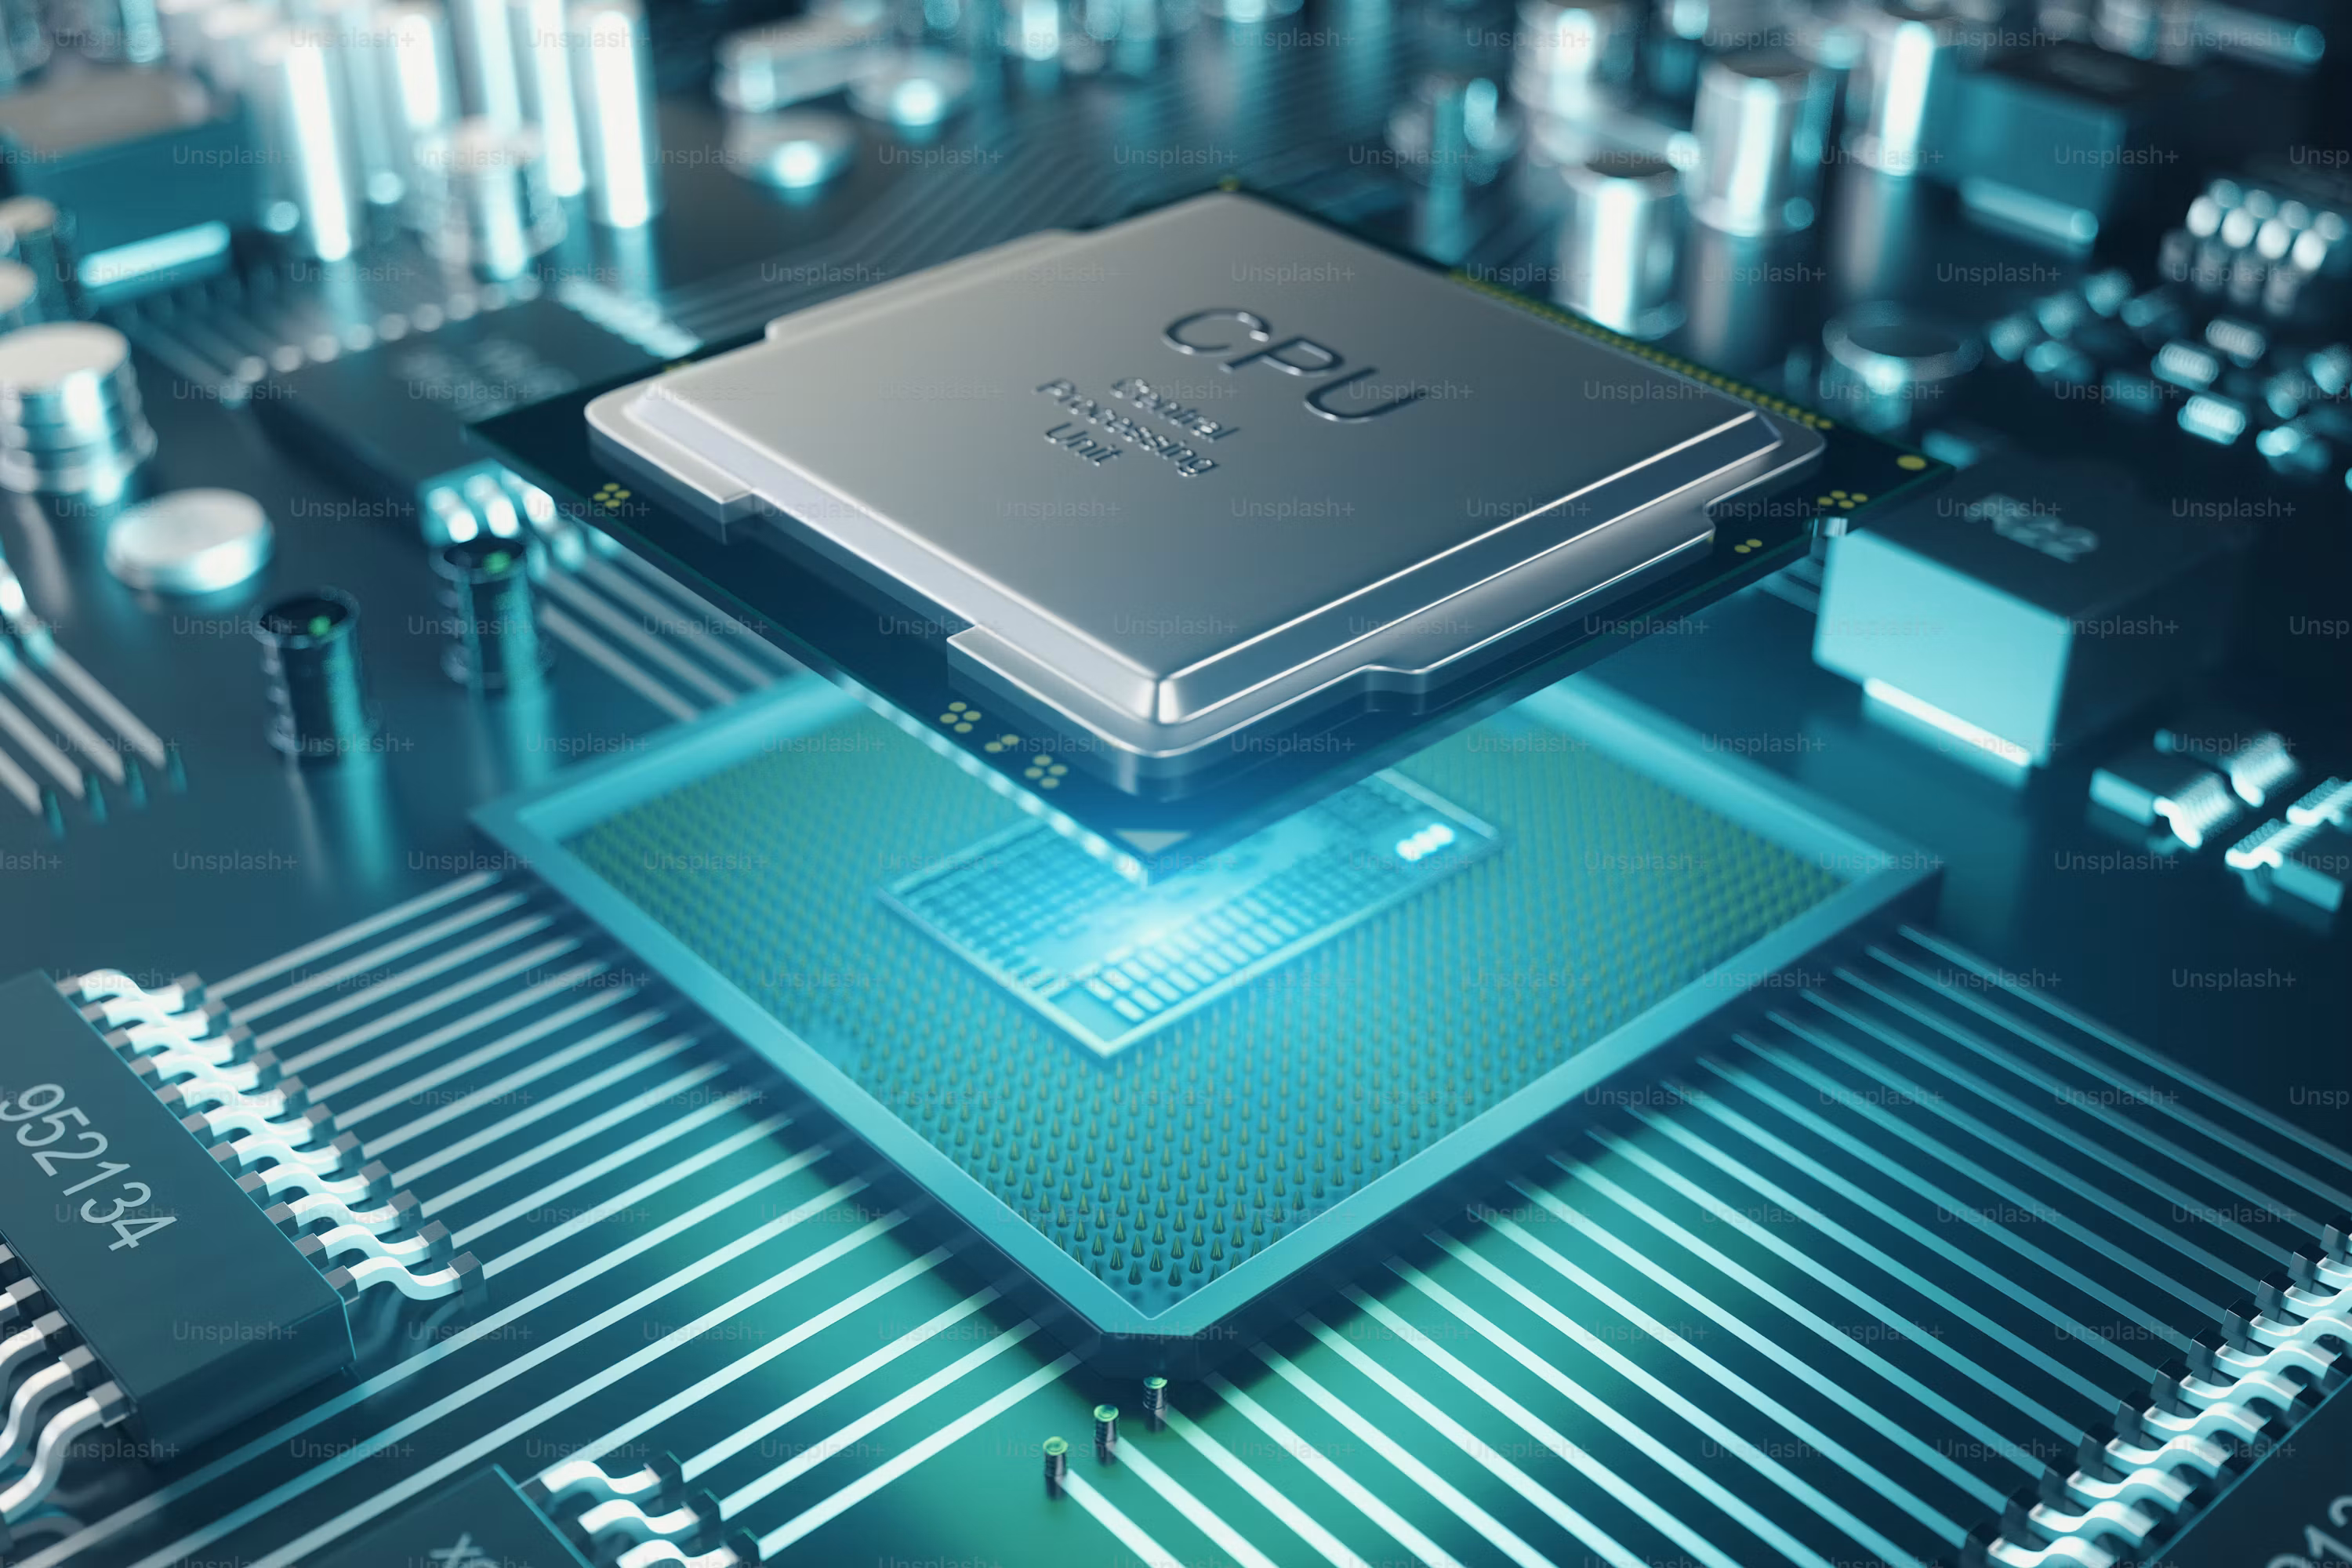
\includegraphics[height=1cm]{Images/top.png}} 
\fancyhead[R]{\thepage} 
\fancyhead[C]{\textit{\leftmark}} 

% Per avere l'intestazione anche nelle pagine iniziali dei capitoli
\fancypagestyle{plain}{
  \fancyhf{}
  \fancyhead[L]{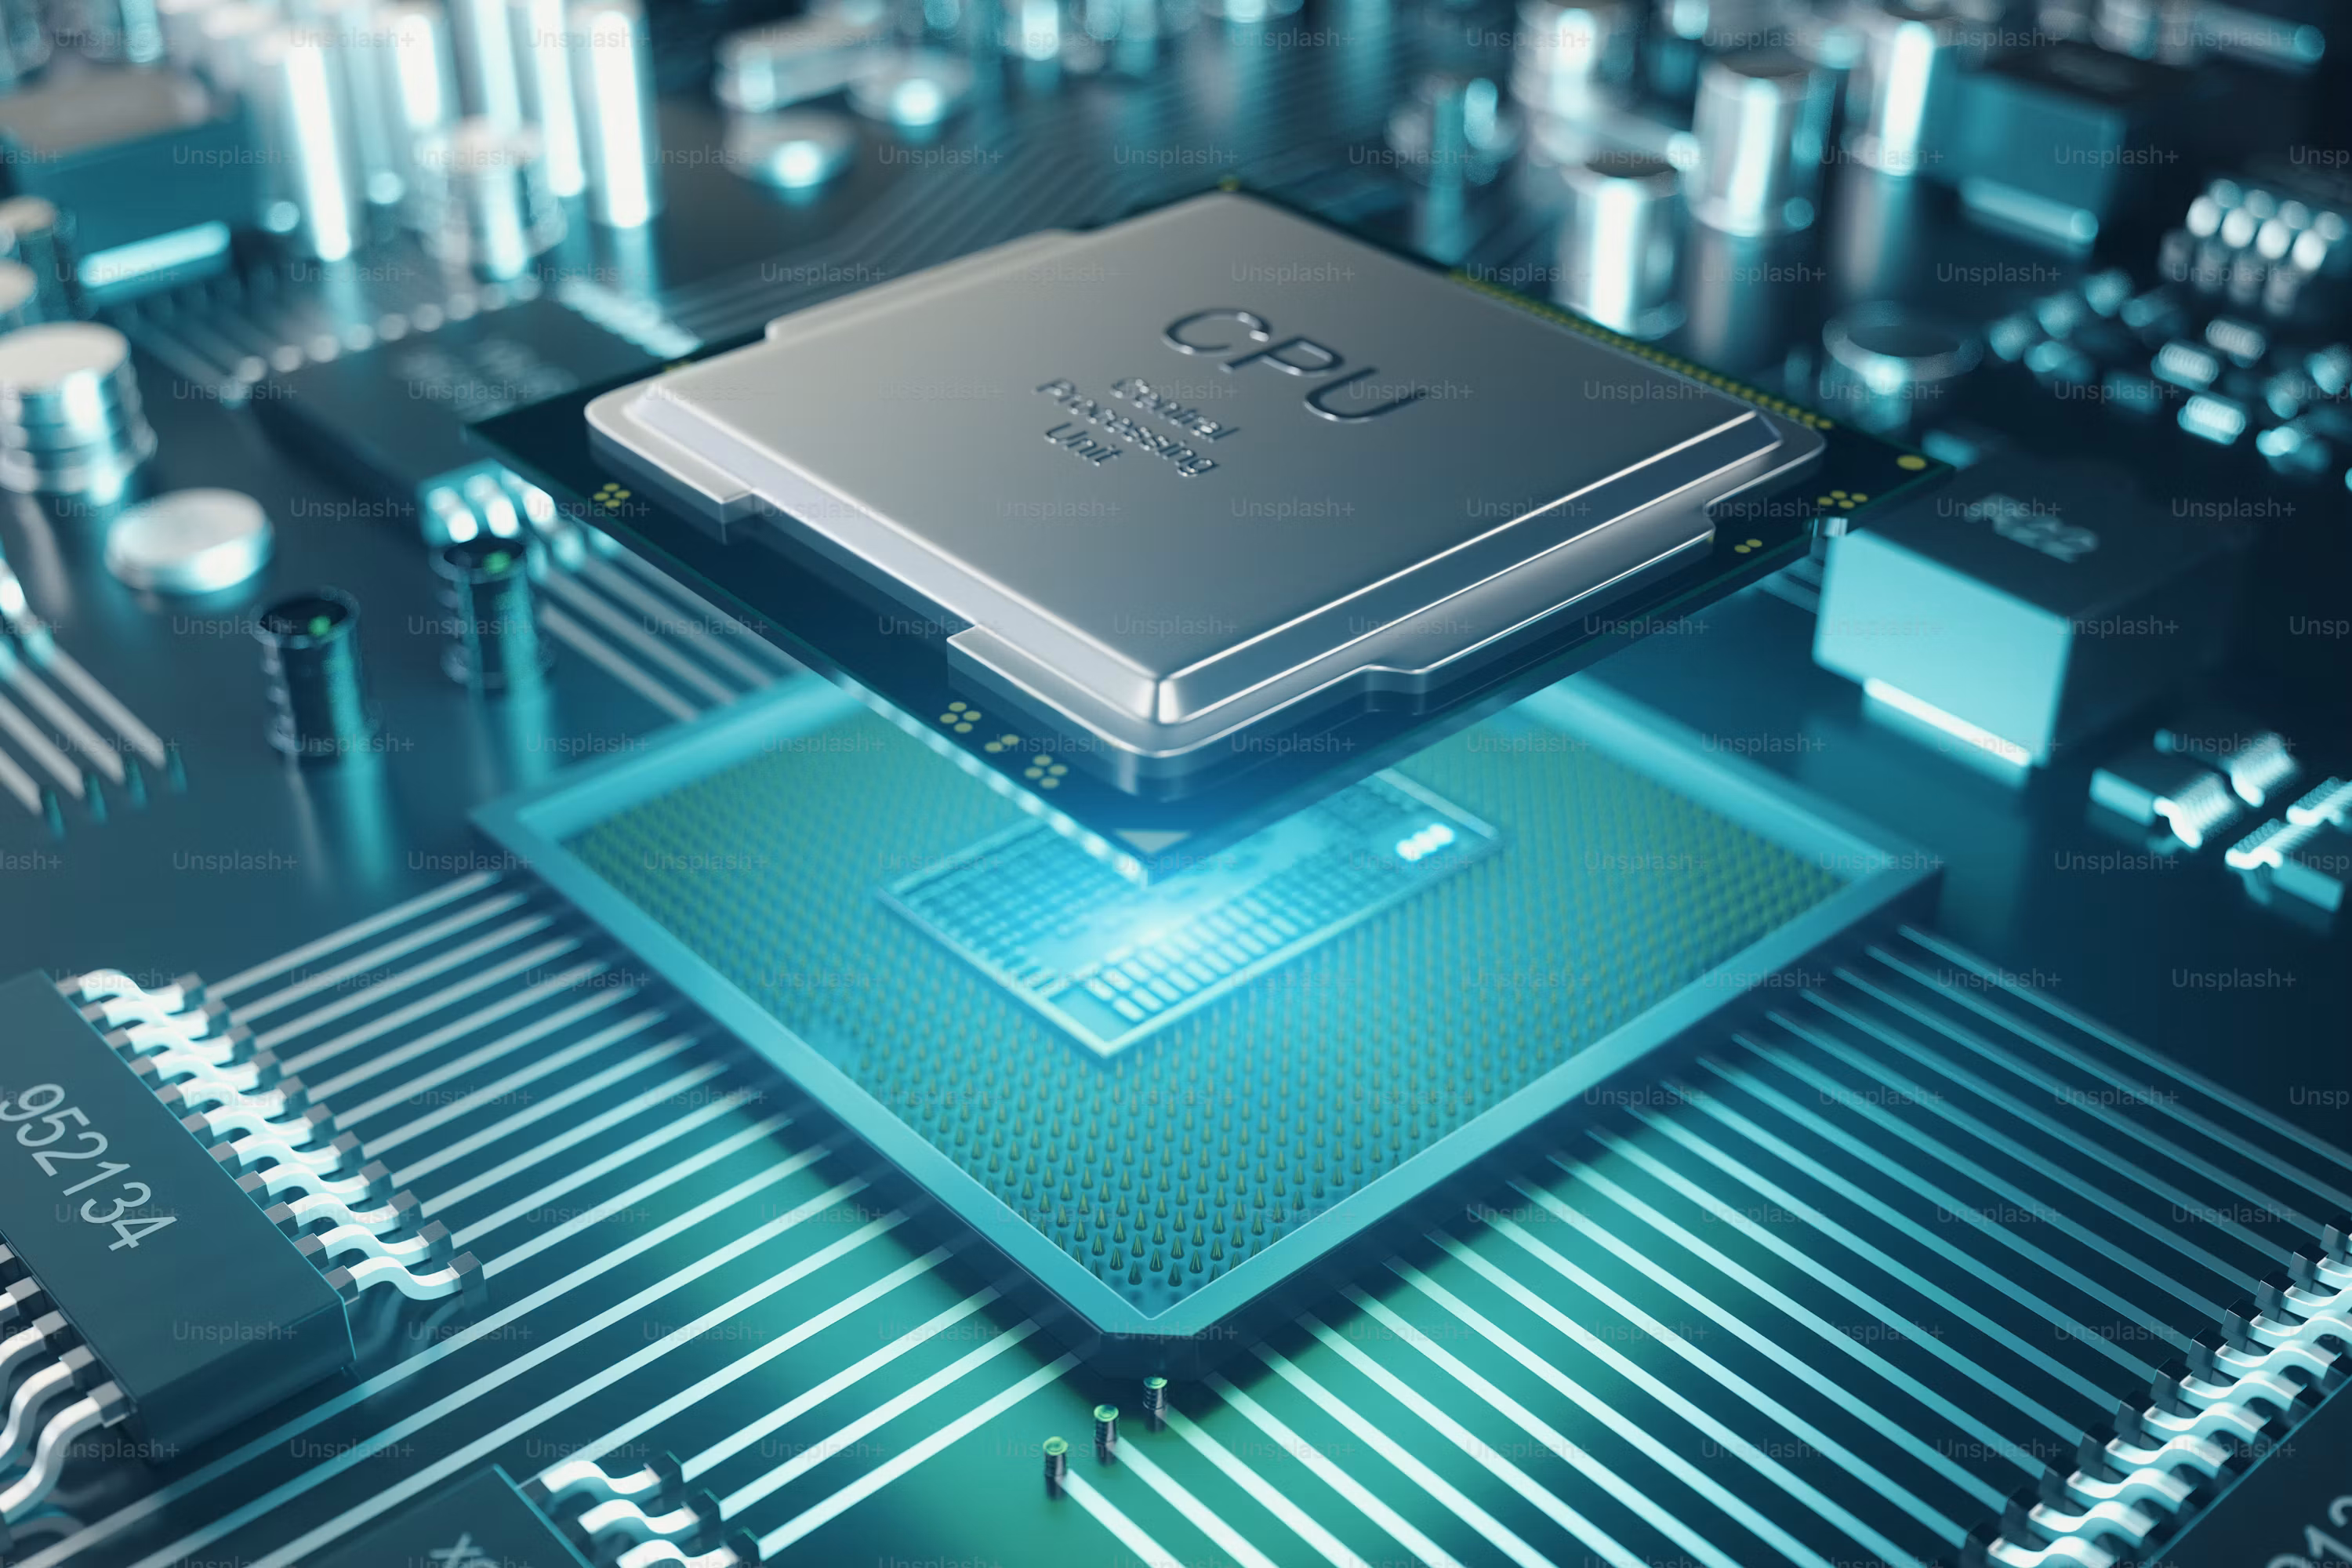
\includegraphics[height=1cm]{Images/top.png}}
  \fancyhead[R]{\thepage}
  \fancyhead[C]{\textit{\leftmark}}
  \renewcommand{\headrulewidth}{0.4pt}
}

% --- LINK CLICCABILI (Senza il backtick d'errore) ---
\usepackage[hidelinks]{hyperref} 
 

% --- COMANDI PERSONALIZZATI ---
\newcommand{\tikznode}[2]{%
  \ifmmode%
    \tikz[remember picture,baseline=(#1.base),inner sep=0pt] \node (#1) {$#2$};%
  \else
    \tikz[remember picture,baseline=(#1.base),inner sep=0pt] \node (#1) {#2};%
  \fi%
}
\tikzset{portnode/.style={circle, draw, inner sep=1pt, font=\scriptsize}}
